%! TEX program = pdflatex

\documentclass[oneside,solution]{seu-ml-assign}

\title{Assignment}
\author{Xie xing}
\studentID{58122204}
\instructor{Xu-Ying Liu}
\date{\today}
\duedate{May 31, 2024}
\assignno{4}
\semester{SEU --- 2024 Spring}
\mainproblem{Support Vector Machine \& Bayesian Classifiers}

\begin{document}

\maketitle

% \startsolution[print]
%第一题SVM
\problem{Support Vector Machine }

%第一题第一问
\subsection{}


%第一题第一问(a)
\subsubsection{(a)}
Generalized Lagrangian function:
\begin{equation}\begin{aligned}             & L(\omega,b,\epsilon,\alpha,\mu)=\frac12||\omega||^2+C\sum_{i=1}^N\epsilon_i,-\sum_{i=1}^N
                           \alpha_i(y_i(\omega^Tx_i+b) -1 + \epsilon)-\sum_{i=1}^N\mu_i\epsilon_i\end{aligned}
\end{equation},
where $ \alpha_i >= 0, \mu_i >=0$.
% The dual problem is the minimax problem of the Lagrangian function, now we firstly calcuate the partial derivative of the Lagrangian function:
The dual problem of the original function is
\begin{equation}\max_{\alpha\geq0,\mu\geq0}\min_{\omega,b,\epsilon}L(\omega,b,\epsilon,\alpha,\mu)\end{equation}

Find the partial derivative :
\begin{equation}
  \nabla_{w}L(w,b,\epsilon,\alpha,\mu)=w-\sum_{i=1}^{N}\alpha_{i}y_{i}x_{i}=0
\end{equation}

\begin{equation}
  \nabla_{b}L(w,b,\epsilon,\alpha,\mu)=-\sum_{i=1}^{N}\alpha_{i}y_{i}=0
\end{equation}

\begin{equation}
  \nabla_{\epsilon_{i}}L(w,b,\epsilon,\alpha,\mu)=C-\alpha_{i}-\mu_{i}=0
\end{equation}

Solutions have to:
\begin{equation}\left.\left\{\begin{aligned}w                       & =\sum_{i=1}^N\alpha_iy_ix_i \\
               \sum_{i=1}^N\alpha_iy_i & =0                          \\
               C-\alpha_i-\mu_i        & =0\end{aligned}\right.\right.
\end{equation}

Bringing in $L(w,b,\epsilon,\alpha,\mu)$ gets:

\begin{equation}\min_{\omega,b,\epsilon}L(w,b,\epsilon,\alpha,\mu)=-\frac12\sum_{i=1}^N
  \sum_{j=1}^N\alpha_i\alpha_jy_iy_j\left(x_i\cdot x_j\right)+\sum_{i=1}^N\alpha_i
\end{equation}

calcuate the maximum of $\min_{\omega,b,\epsilon}L(w,b,\epsilon,\alpha,\mu)$ on $\alpha$, we get the dual problem:

\begin{equation}
  \max_{\alpha} -\frac{1}{2}\sum_{i}^{N}\sum_{j}^{N}\alpha_i\alpha_jy_iy_j(x_i \cdot x_j)+\sum_{i=1}^{N}\alpha_{i}
\end{equation}

\begin{equation}
  s.t.\sum_{i}^{N}\alpha_iy_i=0
\end{equation}

\begin{equation}
  C-\alpha_i-\mu_i=0
\end{equation}

\begin{equation}
  \alpha_i \geq 0
\end{equation}

\begin{equation}
  \mu_i \geq 0, i = 1,2,...,N
\end{equation}


% Next, we originally found the maximum value of the above equation.
% If we add a negative sign to the entire equation, we can transform it into finding its minimum value, that is,
% \begin{equation}\min_\alpha\frac12\sum_{i=1}^N\sum_{j=1}^N\alpha_i\alpha_ju_iy_j\left(x_i\right.\cdot x_j)-\sum_{i=1}^N\alpha \end{equation}

% After getting the objective function, sort out the constraints.
First of all, there is a partial derivative solution $\sum_{i=1}^N\alpha_iy_i=0$,;\\
Secondly, the Lagrange multiplier is greater than or equal to 0, that is $\alpha, \mu >=0$,
when seeking partial derivatives, we get $C-\alpha_i-\mu_i=0$;\\
Finally, comprehensively we get $0\leq\alpha_i\leq C$.

So the dual problem is:

\begin{equation}
  \max_{\alpha} -\frac{1}{2}\sum_{i}^{N}\sum_{j}^{N}\alpha_i\alpha_jy_iy_j(x_i \cdot x_j)+\sum_{i=1}^{N}\alpha_{i}
\end{equation}

\begin{equation}
  s.t.\sum_{i}^{N}\alpha_iy_i=0
\end{equation}

\begin{equation}
  0\leq \alpha_i \leq C
\end{equation}




%第一题第一问(b)
\subsubsection{(b)}
At the saddle point, the solutions of the primal and dual problems are the same, satisfying the following KKT conditions:

\begin{enumerate}
  \item Primal feasibility condition:
        \begin{equation}
          y_i (w \cdot x_i + b) \geq 1 - \epsilon_i, \quad \epsilon_i \geq 0, \quad \forall i
        \end{equation}
  \item Dual feasibility condition:
        \begin{equation}
          0 \leq \alpha_i \leq C, \quad \forall i
        \end{equation}
  \item Complementary slackness condition:
        \begin{equation}
          \alpha_i [y_i (w \cdot x_i + b) - 1 + \epsilon_i] = 0, \quad \forall i
        \end{equation}
  \item Slack variable condition:
        \begin{equation}
          \mu_i \epsilon_i = 0, \quad \forall i
        \end{equation}
  \item Gradient condition:
        \begin{equation}
          w = \sum_{i=1}^n \alpha_i y_i x_i
        \end{equation}
\end{enumerate}

So the primal problem and the dual problem are strongly dual, thus the dual problem is equivalent to the primal problem when at its saddle point.




%第一题第二问
\subsection{}
%第一题第二问(a)
\subsubsection{(a)}

The corresponding mapping function is:
\begin{equation}\phi(x)=(x_1^2,\sqrt{2}x_1x_2,x_2^2)\end{equation}


%第一题第二问(b)
\subsubsection{(b)}
we use the code as follows:
\begin{lstlisting}[language=Python]
  import numpy as np
  import matplotlib.pyplot as plt
  
  # Create XOR data
  np.random.seed(0)
  X_xor = np.random.randn(40, 2)
  y_xor = np.logical_xor(X_xor[:, 0] > 0, X_xor[:, 1] > 0)
  y_xor = np.where(y_xor, 1, -1)
  
  # Plot original XOR data
  plt.scatter(X_xor[y_xor == 1, 0], X_xor[y_xor == 1, 1], color='g', marker='x', label='1')
  plt.scatter(X_xor[y_xor == -1, 0], X_xor[y_xor == -1, 1], color='b', marker='o', label='-1')
  plt.legend()  # Display legend
  plt.title('Original XOR Data')
  plt.show()
  
  # Mapping function φ(x)
  def phi(x):
      return np.array([x[0]**2, np.sqrt(2)*x[0]*x[1], x[1]**2])
  
  # Apply mapping to the data
  X_mapped = np.array([phi(x) for x in X_xor])
  
  # Plot mapped data
  fig = plt.figure()
  ax = fig.add_subplot(111, projection='3d')
  ax.scatter(X_mapped[y_xor == 1, 0], X_mapped[y_xor == 1, 1], X_mapped[y_xor == 1, 2], color='g', marker='x', label='1')
  ax.scatter(X_mapped[y_xor == -1, 0], X_mapped[y_xor == -1, 1], X_mapped[y_xor == -1, 2], color='b', marker='o', label='-1')
  ax.set_xlabel('x1^2')
  ax.set_ylabel('sqrt(2)x1x2')
  ax.set_zlabel('x2^2')
  plt.legend()  # Display legend
  plt.title('Mapped XOR Data')
  plt.show()  
\end{lstlisting}
\begin{figure}[htbp]
  \centering
  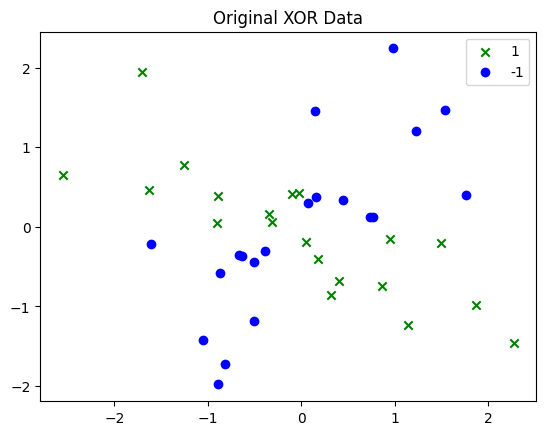
\includegraphics[width=0.6\textwidth]{1.2.b1.png}
  \caption[Original XOR Data]{Original XOR Data}
  \label{1.2.b1}
\end{figure}

\begin{figure}[htbp]
  \centering
  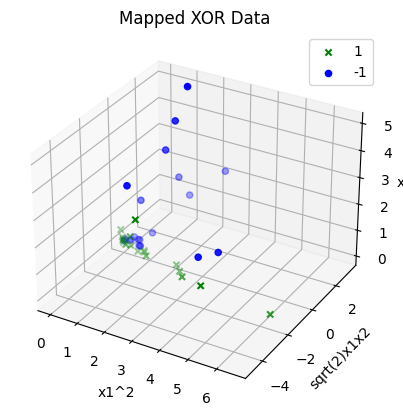
\includegraphics[width=0.6\textwidth]{1.2.b2.png}
  \caption[Mapped XOR Data]{Mapped XOR Data}
  \label{1.2.b2}
\end{figure}
Figure~\ref{1.2.b1} and figure~\ref{1.2.b2} shows the data points in the transformed 3D space using the mapping function $\phi(x)=(x_1^2,\sqrt{2}x_1x_2,x_2^2)$.
In this space, the XOR data points should be linearly separable.

%第一题第二问(c)


\subsubsection{(c)}


The decision boundary in the figure (original feature space) is shown in Figure \ref{1.2.c1}.
\begin{figure}[htbp]
  \centering
  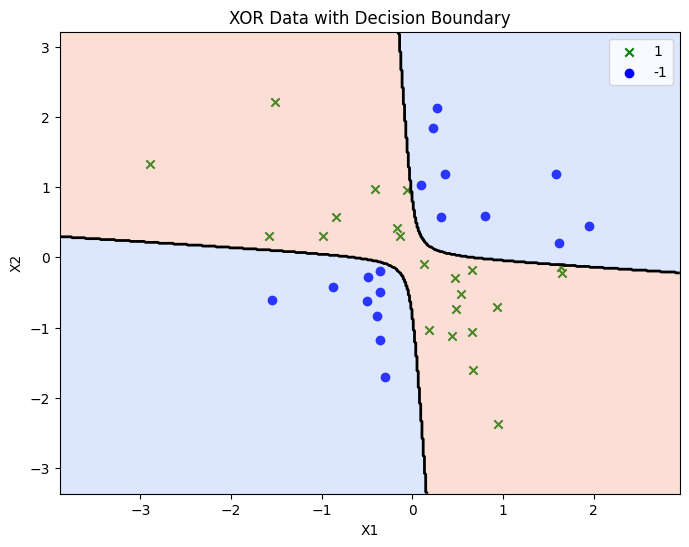
\includegraphics[width=0.6\textwidth]{1.2.c1.png}
  \caption[XOR Data with Decision Boundary]{XOR Data with Decision Boundary}
  \label{1.2.c1}
\end{figure}



The decision boundary in the figure (Regenerative Kernel Hilbert Space) is shown in Figure \ref{1.2.c2}.

\begin{figure}[htbp]
  \centering
  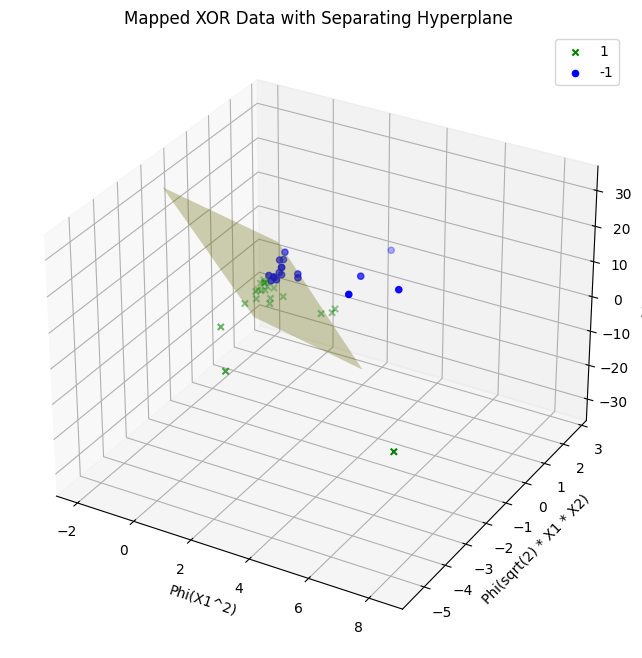
\includegraphics[width=0.6\textwidth]{1.2.c2.png}
  \caption[Mapped XOR Data with Separating Hyperplane]{Mapped XOR Data with Separating Hyperplane}
  \label{1.2.c2}
\end{figure}


\problem{Naïve Bayes Classifier}
\subsection{}
% Empirical Conditional Probabilities with Laplace Smoothing

% For y = +1
\begin{equation}
  P(w = A | y = +1) = \frac{10 + 1}{46 + 4} = \frac{11}{50}
\end{equation}

\begin{equation}
  P(w = B | y = +1) = \frac{5 + 1}{46 + 4} = \frac{6}{50}
\end{equation}

\begin{equation}
  P(w = C | y = +1) = \frac{18 + 1}{46 + 4} = \frac{19}{50}
\end{equation}

\begin{equation}
  P(w = D | y = +1) = \frac{13 + 1}{46 + 4} = \frac{14}{50}
\end{equation}

% For y = -1
\begin{equation}
  P(w = A | y = -1) = \frac{7 + 1}{46 + 4} = \frac{8}{50}
\end{equation}

\begin{equation}
  P(w = B | y = -1) = \frac{11 + 1}{46 + 4} = \frac{12}{50}
\end{equation}

\begin{equation}
  P(w = C | y = -1) = \frac{9 + 1}{46 + 4} = \frac{10}{50}
\end{equation}

\begin{equation}
  P(w = D | y = -1) = \frac{19 + 1}{46 + 4} = \frac{20}{50}
\end{equation}


\subsection{}
% Prediction for New Sample

Given \( A = 3, B = 2, C = 1, D = 2 \):

Calculate the posterior probability for each class \( y \) using the Naïve Bayes formula.

% Prior Probabilities
\begin{equation}
  P(y = +1) = P(y = -1) = \frac{1}{2}
\end{equation}

% Posterior Probabilities

For \( y = +1 \):
\begin{equation}
  P(\mathbf{x} | y = +1) = P(A=3 | y = +1) P(B=2 | y = +1) P(C=1 | y = +1) P(D=2 | y = +1)
\end{equation}

\begin{equation}
  = \left( \frac{11}{50} \right)^3 \left( \frac{6}{50} \right)^2 \left( \frac{19}{50} \right)^1 \left( \frac{14}{50} \right)^2
\end{equation}

For \( y = -1 \):
\begin{equation}
  P(\mathbf{x} | y = -1) = P(A=3 | y = -1) P(B=2 | y = -1) P(C=1 | y = -1) P(D=2 | y = -1)
\end{equation}

\begin{equation}
  = \left( \frac{8}{50} \right)^3 \left( \frac{12}{50} \right)^2 \left( \frac{10}{50} \right)^1 \left( \frac{20}{50} \right)^2
\end{equation}

The Naïve Bayes decision rule is to choose the class with the higher posterior probability. Thus:

\begin{equation}
  \hat{y} = \arg\max_{y} \left( P(y) \cdot P(\mathbf{x} | y) \right)
\end{equation}

For \( y = +1 \):

\begin{equation}
  P(\mathbf{x} | y = +1) P(y = +1) = \frac{1}{2} \cdot \left( \frac{11}{50} \right)^3 \left( \frac{6}{50} \right)^2 \left( \frac{19}{50} \right)^1 \left( \frac{14}{50} \right)^2
\end{equation}

For \( y = -1 \):

\begin{equation}
  P(\mathbf{x} | y = -1) P(y = -1) = \frac{1}{2} \cdot \left( \frac{8}{50} \right)^3 \left( \frac{12}{50} \right)^2 \left( \frac{10}{50} \right)^1 \left( \frac{20}{50} \right)^2
\end{equation}

Compare the two quantities:

\begin{equation}
  \left( \frac{11}{50} \right)^3 \left( \frac{6}{50} \right)^2 \left( \frac{19}{50} \right)^1 \left( \frac{14}{50} \right)^2 < \left( \frac{8}{50} \right)^3 \left( \frac{12}{50} \right)^2 \left( \frac{10}{50} \right)^1 \left( \frac{20}{50} \right)^2
\end{equation}


So $\hat{y} = -1$, namely the label of the new sample where $A=3, B=2, C=1, D=2$ is predicted to be -1.

\problem{Gaussian Bayesian Classifier}

\subsection{}
% Bayes Optimal Classifier
The Bayes optimal classifier that minimizes the misclassification error rate classifies a sample \(\mathbf{x}\) to the class \(y\) with the highest posterior probability \(P(y = k | \mathbf{x})\). This classifier is defined as:

\begin{equation}
  \hat{y}(\mathbf{x}) = \arg\max_{k \in \{1, 2, \ldots, K\}} P(y = k | \mathbf{x})
\end{equation}

Using Bayes' theorem, this can be rewritten as:

\begin{equation}
  \hat{y}(\mathbf{x}) = \arg\max_{k \in \{1, 2, \ldots, K\}} \frac{P(\mathbf{x} | y = k) P(y = k)}{P(\mathbf{x})}
\end{equation}

Since \(P(\mathbf{x})\) is the same for all classes, it simplifies to:

\begin{equation}
  \hat{y}(\mathbf{x}) = \arg\max_{k \in \{1, 2, \ldots, K\}} P(\mathbf{x} | y = k) P(y = k)
\end{equation}


\subsection{}
% Bayes Optimal Classifier for Normal Distribution
Given that the samples in the \(k\)-th class are i.i.d. and follow a normal distribution \(\mathcal{N}(\mu_k, \Sigma)\), the probability density function is:

\begin{equation}
  p(\mathbf{x} | y = k) = \frac{1}{(2\pi)^{d/2} \det(\Sigma)^{1/2}} \exp\left( -\frac{1}{2} (\mathbf{x} - \mu_k)^\top \Sigma^{-1} (\mathbf{x} - \mu_k) \right)
\end{equation}

The prior probability for class \(k\) is \(\pi_k = P(y = k)\). The Bayes optimal classifier is:

\begin{equation}
  \hat{y}(\mathbf{x}) = \arg\max_{k \in \{1, 2, \ldots, K\}} p(\mathbf{x} | y = k) \pi_k
\end{equation}

Substituting the probability density function:

\begin{equation}
  \hat{y}(\mathbf{x}) = \arg\max_{k \in \{1, 2, \ldots, K\}} \frac{1}{(2\pi)^{d/2} \det(\Sigma)^{1/2}} \exp\left( -\frac{1}{2} (\mathbf{x} - \mu_k)^\top \Sigma^{-1} (\mathbf{x} - \mu_k) \right) \pi_k
\end{equation}

Simplifying, we get:

\begin{equation}
  \hat{y}(\mathbf{x}) = \arg\max_{k \in \{1, 2, \ldots, K\}} \exp\left( -\frac{1}{2} (\mathbf{x} - \mu_k)^\top \Sigma^{-1} (\mathbf{x} - \mu_k) \right) \pi_k
\end{equation}

Since the exponential function is monotonically increasing, this can be further simplified to:

\begin{equation}
  \hat{y}(\mathbf{x}) = \arg\max_{k \in \{1, 2, \ldots, K\}} \left( -\frac{1}{2} (\mathbf{x} - \mu_k)^\top \Sigma^{-1} (\mathbf{x} - \mu_k) + \log \pi_k \right)
\end{equation}


\subsection{}
% LDA and Bayes Optimal Classifier for Binary Classification
For the binary classification problem, assume the samples in each class are i.i.d. and follow normal distributions \(\mathcal{N}(\mu_0, \Sigma)\) and \(\mathcal{N}(\mu_1, \Sigma)\) with equal prior probabilities \(\pi_0 = \pi_1\).

The decision rule for LDA is to assign \(\mathbf{x}\) to class 0 if the following discriminant function is greater than zero:

\begin{equation}
  (\mathbf{x} - \frac{\mu_0 + \mu_1}{2})^\top \Sigma^{-1} (\mu_1 - \mu_0) > 0
\end{equation}

This can be derived as follows:

Given the discriminant functions for the two classes, we assign \(\mathbf{x}\) to class 0 if:

\begin{equation}
  p(\mathbf{x} | y = 0) \pi_0 > p(\mathbf{x} | y = 1) \pi_1
\end{equation}

Since \(\pi_0 = \pi_1\), it simplifies to:

\begin{equation}
  p(\mathbf{x} | y = 0) > p(\mathbf{x} | y = 1)
\end{equation}

Taking the logarithm of both sides:

\begin{equation}
  \log p(\mathbf{x} | y = 0) > \log p(\mathbf{x} | y = 1)
\end{equation}

Substituting the normal distribution PDFs:

\begin{equation}
  -\frac{1}{2} (\mathbf{x} - \mu_0)^\top \Sigma^{-1} (\mathbf{x} - \mu_0) > -\frac{1}{2} (\mathbf{x} - \mu_1)^\top \Sigma^{-1} (\mathbf{x} - \mu_1)
\end{equation}

Simplifying this inequality, we get:

\begin{equation}
  (\mathbf{x} - \mu_0)^\top \Sigma^{-1} (\mathbf{x} - \mu_0) < (\mathbf{x} - \mu_1)^\top \Sigma^{-1} (\mathbf{x} - \mu_1)
\end{equation}

This can be rewritten as:

\begin{equation}
  2\mathbf{x}^\top \Sigma^{-1} (\mu_1 - \mu_0) > \mu_1^\top \Sigma^{-1} \mu_1 - \mu_0^\top \Sigma^{-1} \mu_0
\end{equation}

Finally, the decision rule for LDA is:

\begin{equation}
  \mathbf{x}^\top \Sigma^{-1} (\mu_1 - \mu_0) > \frac{1}{2} (\mu_1^\top \Sigma^{-1} \mu_1 - \mu_0^\top \Sigma^{-1} \mu_0)
\end{equation}

Given \( w = \Sigma^{-1} (\mu_1 - \mu_0) \):

\begin{equation}
  \mathbf{x}^\top w > \frac{1}{2} (\mu_1^\top \Sigma^{-1} \mu_1 - \mu_0^\top \Sigma^{-1} \mu_0)
\end{equation}

This shows that the LDA decision rule corresponds to the Bayes optimal classifier under the given assumptions.


\problem{MLE and Linear Regression}
\subsection{}
% Maximum Likelihood Estimation (MLE)
Given that \(\epsilon_i \sim \mathcal{N}(0, \sigma_i^2)\), the probability density function of \(y_i\) given \(X_i\) is:

\begin{equation}
  p(y_i | X_i, f) = \frac{1}{\sqrt{2\pi\sigma_i^2}} \exp\left(-\frac{(y_i - f(X_i))^2}{2\sigma_i^2}\right)
\end{equation}

The likelihood of all observations \(y\) given \(X\) and \(f\) is the product of the individual densities:

\begin{equation}
  L(y | X, f) = \prod_{i=1}^n \frac{1}{\sqrt{2\pi\sigma_i^2}} \exp\left(-\frac{(y_i - f(X_i))^2}{2\sigma_i^2}\right)
\end{equation}

The log-likelihood function is:

\begin{equation}
  \log L(y | X, f) = \sum_{i=1}^n \left( -\frac{1}{2} \log(2\pi\sigma_i^2) - \frac{(y_i - f(X_i))^2}{2\sigma_i^2} \right)
\end{equation}

Maximizing the log-likelihood is equivalent to minimizing the negative log-likelihood:

\begin{equation}
  \text{Minimize: } \sum_{i=1}^n \left( \frac{(y_i - f(X_i))^2}{2\sigma_i^2} \right)
\end{equation}


\subsection{}
% Linear Regression
Assuming a linear relationship \( f(X_i) = w \cdot X_i \), where \( w \) is a \( p \)-dimensional vector of weights, we substitute this into our objective function:

\begin{equation}
  \text{Minimize: } \sum_{i=1}^n \frac{(y_i - w \cdot X_i)^2}{2\sigma_i^2}
\end{equation}

To express this in matrix notation, let's define:
\begin{enumerate}
  \item \( y \) as the \( n \)-dimensional vector of labels.
  \item \( X \) as the \( n \times p \) design matrix.
  \item \( w \) as the \( p \)-dimensional vector of weights.
  \item \( \Sigma \) as a diagonal matrix with \( \sigma_i^2 \) on the diagonal.
\end{enumerate}

The cost function can be written as:

\begin{equation}
  J(w) = \frac{1}{2} (y - Xw)^T \Sigma^{-1} (y - Xw)
\end{equation}

Here, \( \Sigma \) is the diagonal matrix of noise variances \( \sigma_i^2 \).


\subsection{}
% Solution to the Optimization Problem
To find the optimal \( w \), we take the gradient of \( J(w) \) with respect to \( w \) and set it to zero:

\begin{equation}
  \nabla_w J(w) = -X^T \Sigma^{-1} (y - Xw)
\end{equation}

Setting the gradient to zero gives:

\begin{equation}
  X^T \Sigma^{-1} (y - Xw) = 0
\end{equation}

Solving for \( w \):

\begin{equation}
  X^T \Sigma^{-1} X w = X^T \Sigma^{-1} y
\end{equation}

Thus, the solution to the optimization problem is:

\begin{equation}
  w = (X^T \Sigma^{-1} X)^{-1} X^T \Sigma^{-1} y
\end{equation}


\vspace{2mm}
\end{document}
